









\section{\methodshort: \method}

\emph{Quantization} maps a floating-point number into lower-bit integers. It is an effective method to reduce the model size and inference costs of LLMs~\cite{dettmers2022llmint8, frantar2022gptq, zeroquant, xiao2022smoothquant}. In this section, we first propose a weight-only quantization method to improve accuracy \emph{without training/regression} by protecting more ``important'' weights. And then develop a data-driven method to search for the optimal scaling that reduces quantization errors (Figure~\ref{fig:overview}). 

\subsection{Improving LLM Quantization by Preserving 1\% Salient Weights}
\renewcommand \arraystretch{1.05}
\begin{table*}[t]
    \setlength{\tabcolsep}{4.5pt}
    \small
    \centering
    \vspace{5pt}
    \begin{tabular}{lccccccccccc}
        \toprule
          \multirow{2}{*}{\textbf{PPL $\downarrow$}}   & \multirow{2}{*}{FP16} & \multirow{2}{*}{RTN}   & \multicolumn{3}{c}{FP16\% (based on act.)}  & \multicolumn{3}{c}{FP16\% (based on W)} &  \multicolumn{3}{c}{FP16\% (random)} \\ \cmidrule(lr){4-6} \cmidrule(lr){7-9}  \cmidrule(lr){10-12}
         & & (w3-g128) & 0.1\% & 1\% & 3\% &   0.1\% & 1\% & 3\% &  0.1\% & 1\% & 3\%   \\
        \midrule
        OPT-1.3B  & 14.62 & 119.00 & 25.03 & \textcolor{codegreen}{16.91} & \textcolor{codegreen}{16.68} & 108.71 & 98.55 & 98.08 & 119.76 & 109.38 & 61.49 \\
        OPT-6.7B & 10.86 & 23.54 & \textcolor{codegreen}{11.58} & \textcolor{codegreen}{11.39} & \textcolor{codegreen}{11.36} & 23.41 & 22.37 & 22.45 & 23.54 & 24.23 & 24.22 \\
        OPT-13B &  10.13 & 46.04 &\textcolor{codegreen}{10.51} & \textcolor{codegreen}{10.43} & \textcolor{codegreen}{10.42} & 46.07 & 48.96 & 54.49 & 44.87 & 42.00 & 39.71 \\
        \bottomrule
    \end{tabular}
    \caption{Keeping a small fraction of weights (0.1\%-1\%) in FP16 significantly improves the performance of the quantized models over round-to-nearest (RTN). It is only effective when we select the important weights in FP16 by looking at \emph{activation} distribution instead of \emph{weight} distribution. We highlight results with a decent perplexity in \textcolor{codegreen}{green}.  
    We used INT3 quantization with a group size of 128 and measured the WikiText perplexity ($\downarrow$).  
    } 
    \label{tab:fp_ratio}
\end{table*}


We observe that the weights of LLMs are \emph{not equally important}: there is a small fraction of \emph{salient} weights that are much more important for LLMs' performance compared to others. Skipping the quantization of these salient weights can help bridge the performance degradation due to the quantization loss \emph{without} any training or regression (Figure~\ref{fig:overview}(b)).
To verify the idea, we benchmark the performance of quantized LLMs when skipping part of the weight channels in Table~\ref{tab:fp_ratio}. We measured the performance of INT3 quantized models while keeping some ratios of weight channels in FP16. A widely used method to determine the importance of weights is to look at its magnitude or $L_2$-norm~\cite{han2015learning, frankle2018lottery}. But we find skipping the weight channels with large norm (\ie, FP16\% (based on W)) does not significantly improve the quantized performance, leading to a similar marginal improvement as random selection. 
Interestingly, selecting weights based on \emph{activation magnitude} can significantly improve the performance despite keeping only 0.1\%-1\% of channels in FP16. 
We hypothesize that the input features with larger magnitudes are generally more important. Keeping the corresponding weights in FP16 can preserve those features, which contributes to better model performance. 

\textbf{Limitations: }
Despite keeping 0.1\% of weights in FP16 can improve the quantized performance without a noticeable increase in model size (measured in total bits), such a mixed-precision data type will make the system implementation difficult. We need to come up with a method to protect the important weights without actually keeping them as FP16. 


\subsection{Protecting Salient Weights by Activation-aware Scaling}
We propose an alternative method to reduce the quantization error of the salient weight by \emph{per-channel scaling}, which does not suffer from the hardware inefficiency issue. 

\textbf{Analyzing the quantization error.}




\begin{table}
    \setlength{\tabcolsep}{2pt}
    \small
    \centering
    \begin{tabular}{lccccc}
        \toprule
     \textbf{OPT-6.7B}   & $s=1$ & $s=1.25$ & $s=1.5$ & $s=2$ & $s=4$ \\ \midrule
    proportion of $\Delta^{'} \neq \Delta$ & 0\% & 2.8\% & 4.4\% & 8.2\% & 21.2\% \\
    average $\Delta^{'}/ \Delta$ & 1 & 1.005 & 1.013 & 1.038 & 1.213 \\
    average $\frac{\Delta^{'}}{\Delta} \cdot \frac{1}{s}$ & 1 & 0.804  & 0.676 & 0.519 & \textbf{0.303} \\ \midrule 
    Wiki-2 PPL & 23.54 & 12.87 & 12.48 & \textbf{11.92} & 12.36 \\
    \bottomrule
    \end{tabular}
    \caption{Statistics when multiplying the 1\% salient channels by $s>1$. Scaling up the salient channels significantly improves the perplexity (23.54 to 11.92). As $s$ goes larger, the percentage of changed $\Delta$ increases, and the error reduction rate for salient channels also increases. However, the best perplexity is achieved at $s=2$, since further increasing $s$ will increase the quantization error for \emph{non-salient} channels. 
    } 
    \label{tab:scale_study}
\end{table}


We start by analyzing the error from weight-only quantization. 
Consider a group/block of weight $\mathbf{w}$; the linear operation can be written as $y=\mathbf{w}\mathbf{x}$, and the quantized counterpart is $y=Q(\mathbf{w})\mathbf{x}$. Specifically, the quantization function is defined as:
\begin{equation}
    Q(\mathbf{w}) = \Delta \cdot \text{Round}(\frac{\mathbf{w}}{\Delta}), \quad \Delta = \frac{\max(|\mathbf{w}|)}{2^{N-1}},
    \label{eq:org_quant}
\end{equation}
where $N$ is the number of quantization bits, and $\Delta$ is the quantization scaler determined by the absolute maximum value. Now consider a weight element $w\in \mathbf{w}$, if we multiply $w$ with $s> 1$ and the inversely scale $x$, we will have $Q(w\cdot s)(x/s)$, which is:
\begin{equation}
    Q(w\cdot s)\cdot \frac{x}{s} = \Delta^{'} \cdot \text{Round}(\frac{ws}{\Delta^{'}}) \cdot x \cdot \frac{1}{s},
    \label{eq:scaled_quant}
\end{equation}
where $\Delta^{'}$ is the new quantization scaler after applying $s$. We empirically find that: (1) The expected error from $\text{Round}(\cdot)$ (denoted as $\texttt{RoundErr}(\cdot)$) does not change: since the round function maps a floating-point number to an integer, the error is roughly uniformly distributed from [0,0.5], resulting in an average error of $0.25$; i.e., $\texttt{RoundErr}(\cdot)\sim 0.25$. (2) Scaling up a single element $w$ usually does not change the maximum value from the group $\mathbf{w}$. Therefore we have $\Delta^{'}\approx\Delta$;
(3) As $\Delta$ and $x$ are represented in FP16, they have no quantization error. Consequently, the quantization error from equation~\ref{eq:org_quant} and ~\ref{eq:scaled_quant} can be expressed as 
\begin{equation}
\begin{aligned}
\texttt{Err}(Q(w) x) &= \Delta\cdot \texttt{RoundErr}(\frac{w}{\Delta})\cdot x \\
\texttt{Err}(Q(w \cdot s)(\frac{x}{s})) &= \Delta^{'}\cdot \texttt{RoundErr}(\frac{ws}{\Delta^{'}})\cdot x\cdot \frac{1}{s}
\end{aligned}
\end{equation}
The ratio of the new error to the original error is $\frac{\Delta^{'}}{\Delta} \cdot \frac{1}{s}$. Given $\Delta^{'}\approx\Delta$ and $s>1$, the relative error is smaller for the salient weight $w$. 


To verify the idea, we multiply the 1\% salient channels with $s>1$ for the OPT-6.7B model, and measure the change in $\Delta$ for each group in Table \ref{tab:scale_study}. We find that scaling up the salient channels is quite effective: the perplexity improves from 23.54 for $s=1$ (simply RTN) to 11.92 for $s=2$. 
As $s$ goes larger, the percentage of changed $\Delta$ generally gets larger, but the percentage is still quite small for $s<2$ (less than 5\%); the relative error for the salient channels continues to go smaller as $s$ increases. Nonetheless, the best PPL actually appears at $s=2$. This is because if we use a very large $s$, it will increase the relative error for the \emph{non-salient} channels when $\Delta$ increases (the error of non-salient channels will be amplified by $\frac{\Delta^{'}}{\Delta}$, and the ratio is larger than 1 for 21.2\% of the channels under $s=4$), which can damage the model's overall accuracy. Therefore, we need to also consider the error from non-salient channels when protecting salient ones. 





\begin{table}
    \setlength{\tabcolsep}{5pt}
    \small
    \centering
    \begin{tabular}{llccccccc}
      \toprule
        \textbf{OPT (PPL}$\downarrow$) & 1.3B & 2.7B & 6.7B  & 13B & 30B   \\  \midrule
      FP16 & 14.62 & 12.47 & 10.86 & 10.13	& 9.56 \\ \midrule
      RTN & 119.47 & 298.00 & 23.54 & 46.04	& 18.80	 \\
       1\% FP16 & 16.91 & 13.69 & \textbf{11.39} & \textbf{10.43} & 9.85 \\
       $s=2$ & 18.63 & 14.94 & 11.92 & 10.80 & 10.32 \\
       \methodshort  &  \textbf{16.32} & \textbf{13.58} &\textbf{11.39} & 10.56 & \textbf{9.77}	\\
      \bottomrule
    \end{tabular}
    \caption{\methodshort protects salient weights and reduces quantization error by using a scaling-based method. It consistently outperforms Round-to-nearest quantization (RTN) and achieves comparable performance as mixed-precision (1\% FP16) while being more hardware-friendly. We use 3-bit quantization with group size 128.}
    \label{tab:opt_ppl}
\end{table}



\begin{figure*}[t]
    \centering
     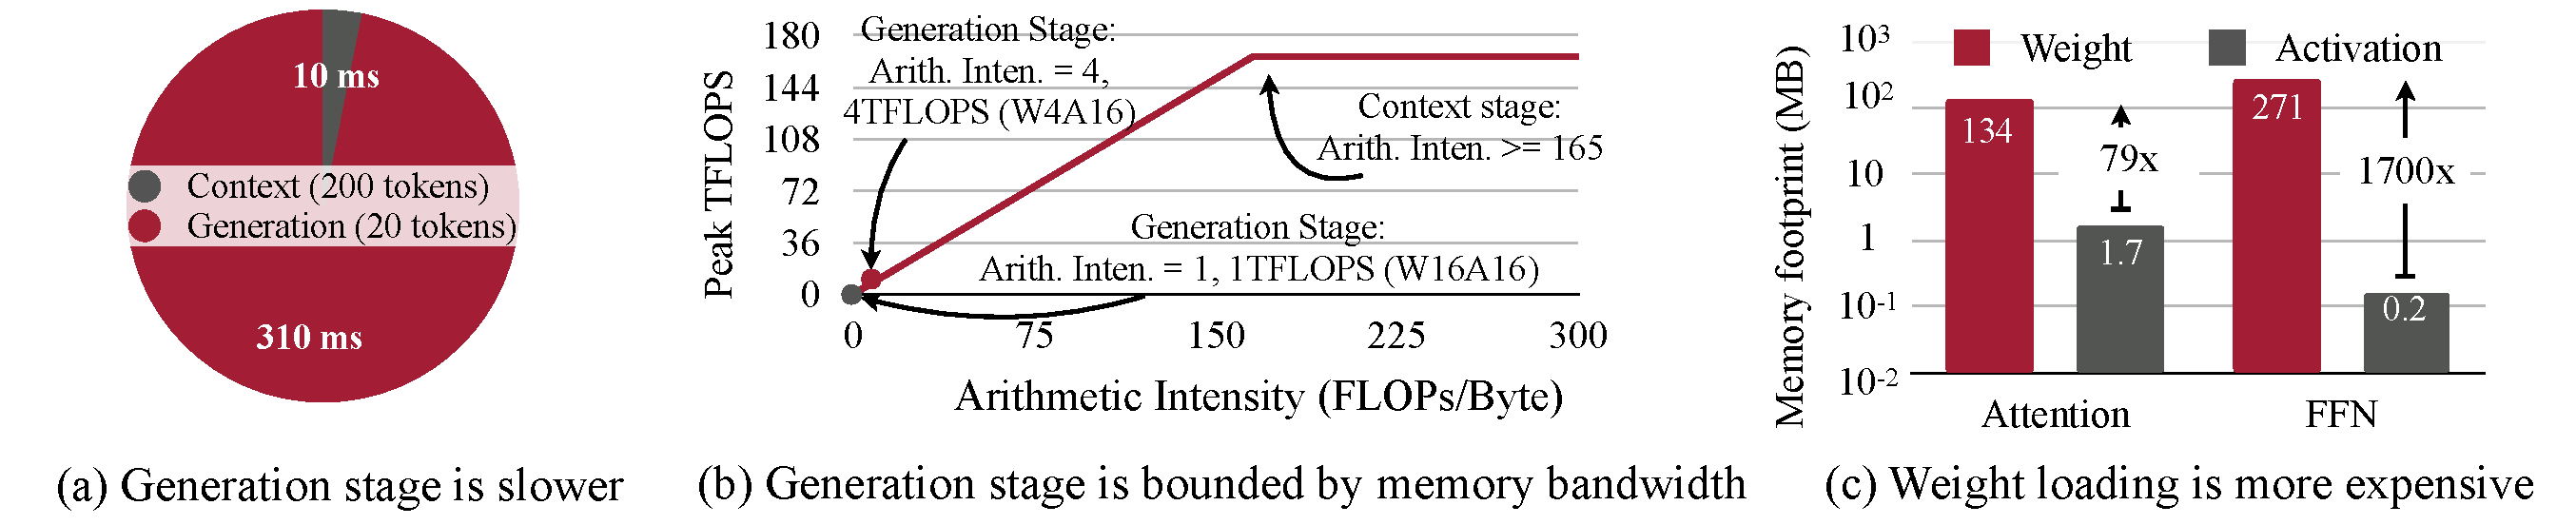
\includegraphics[width=\textwidth]{figures/memory_bound_analysis.pdf}
    \caption{Bottleneck analysis for Llama-2-7B on NVIDIA RTX 4090. \textbf{Left}: In on-device LLM applications, generation stage is much slower than the context stage. \textbf{Middle}: The generation stage is memory bound and has low arithmetic intensity. W4A16 quantization can effectively improve the arithmetic intensity by 4$\times$. \textbf{Right}: The amount of weight access is orders of magnitude larger than the amount of activation access. Thus, weight-only quantization is more effective for on-device LLMs.} 
    \label{fig:memory_bound_analysis}
\end{figure*}


\textbf{Searching to scale. }
To consider both salient and non-salient weights, we choose to automatically search for an optimal (per input channel) scaling factor that minimizes the output difference after quantization for a certain layer. Formally, we want to optimize the following objective:
\begin{equation}
\begin{aligned}
    \mathbf{s}^* &= \mathop{\arg\min}_{\mathbf{s}} \mathcal{L}(\mathbf{s}) \\  
    \mathcal{L}(\mathbf{s}) = \lVert Q(\mathbf{W}\cdot \text{di}&\text{ag}(\mathbf{s}))  (\mathbf{\text{diag}(s)^{-1}} \cdot \mathbf{X}) - \mathbf{W}\mathbf{X}  \rVert
\end{aligned}
\end{equation}
Here $Q$ means the weight quantization function (\eg, INT3/INT4 quantization with group size 128), $\mathbf{W}$ is the original weights in FP16, and $\mathbf{X}$ is the input features cached from a small calibration set (we take a small calibration set from he pre-training dataset in order not to overfit to a specific task). $\mathbf{s}$ is a per-(input) channel scaling factor; for $\mathbf{s^{-1}} \cdot \mathbf{X}$, it can usually be fused into the previous operator~\cite{wei2022outlier, xiao2022smoothquant}.
Since the quantization function is not differentiable, we are not able to directly optimize the problem with vanilla backpropagation. There are some techniques relying on approximated gradients~\cite{bengio2013estimating, esser2019learned}, which we found still suffers from unstable convergence.  

To make the process more stable, we define a \emph{search space} for the optimal scale by analyzing the factors that will affect the choice of scaling factor. As shown in the last section, the saliency of weight channels is actually determined by the activation scale (thus ``activation-awareness''). Therefore, we simply use a very simple search space:
\begin{equation}
\label{eq:scale_search_formula}
    \mathbf{s}=\mathbf{s_X}^{\alpha}, \quad \alpha^*=\mathop{\arg\min}_{\alpha}\mathcal{L}(\mathbf{s_X}^{\alpha})
\end{equation}
$\mathbf{s_X}$ is the average magnitude of activation (per-channel), and we use a single hyper-parameter $\alpha$ to balance between the protection of salient and non-salient channels. We can find the best $\alpha$ by a fast grid search over the interval of $[0, 1]$ ($0$ means we do not scale; $1$  corresponds to the most aggressive scaling in our search space). We further apply weight clipping to minimize the MSE error of quantization. We provide an ablation study on OPT models under INT3-g128 quantization in Table~\ref{tab:opt_ppl}; \methodshort consistently outperforms round-to-nearest quantization (RTN) and achieves comparable performance as mixed-precision (1\% FP16) while being more hardware-friendly.



\textbf{Advantages.} 
Our method does not rely on any regression~\cite{frantar2022gptq} or backpropagation, which is required by many quantization-aware training methods. It has minimal reliance on the calibration set since we only measure the average magnitude per channel, thus preventing over-fitting (Figure~\ref{fig:calib_set_ablation}). Therefore, our method requires fewer data for the quantization process and can preserve LLMs' knowledge outside of the calibration set's distribution. 
See Section~\ref{sec:ablation_study} for more details. %
















